\begin{name}
	{\tenchude}{\tendethi}{LỚP TOÁN THẦY PHÁT}{\thoigian}
\end{name}
	\setcounter{ex}{0}\setcounter{bt}{0}
	\Opensolutionfile{ans}[ans/ans-2-TT-6-THPTChuyenVinhPhuc-L2-23]
	
\begin{ex}%[Kiểm tra chuyên đề lần 2, THPT Chuyên Vĩnh Phúc Lần 2, 2023]%[Đăng Tạ, 12EX6]%[1D2B1-2]
	Từ các chữ số $1$, $2$, $3$, $4$, $5$, $6$, $7$ có thể lập được bao nhiêu số có bốn chữ số chia hết cho $2$?
	\choice
	{$1149$}
	{\True $1029$}
	{$574$}
	{$2058$}
	\loigiai{
		Gọi số chia hết cho $2$ có bốn chữ số là $\overline{a_1a_2a_3a_4}$. Điều kiện $a_i \neq a_j$ với $i\neq j$ và $a_4$ chẵn.
		\begin{itemize}
			\item Chọn $a_4$ có $3$ cách $\left(a_4\in \{2;4;6\}\right)$.
			\item Chọn $a_1$ có $7$ cách chọn.
			\item Chọn $a_2$ có $7$ cách chọn.
			\item Chọn $a_3$ có $7$ cách chọn.
		\end{itemize}
		Vậy có $3\cdot 7\cdot 7\cdot 7=1029$ số thỏa.
	}
\end{ex}

\begin{ex}%[Kiểm tra chuyên đề lần 2, THPT Chuyên Vĩnh Phúc Lần 2, 2023]%[Đăng Tạ, 12EX6]%[1D3T3-6] 
	Biết rằng mức lương của một kỹ sư ở công ty X trong quý I năm $2017$ ($3$ tháng đầu tiên của năm $2017$) là $S_0$ (triệu đồng), kể từ quý II mức lương sẽ được tăng thêm $0,5$ triệu đồng mỗi quý. Tổng lương của kỹ sư đó tính từ quý I năm $2017$ đến hết quý IV năm $2022$ là $1002$ (triệu đồng). Tính tổng lương $S$ (triệu đồng) của kỹ sư tính từ quý I năm $2017$ đến hết quý IV năm $2025$.
	\choice
	{$S=1911$}
	{$S=324$}
	{\True $S=1611$}
	{$S=342$}
	\loigiai{
		Tổng lương là tổng của cấp số cộng có $u_1=S_0$, $d=0{,}5$.\\
		Tổng lương của kỹ sư đó tính từ quý I năm $2017$ đến hết quý IV năm $2022$ (gồm 24 quý) là 
		$$1002=24u_1+\dfrac{24(24-1)}{2}0{,5}\Leftrightarrow u_1=36.$$
		Tổng lương của kỹ sư đó tính từ quý I năm $2017$ đến hết quý IV năm $2025$ (gồm 36 quý) là 
		$$S=36\cdot 36+\dfrac{36(36-1)}{2}0{,5}=1611.$$
	}
\end{ex}

\begin{ex}%[Kiểm tra chuyên đề lần 2, THPT Chuyên Vĩnh Phúc Lần 2, 2023]%[Đăng Tạ, 12EX6]%[2H2Y1-2] 
	Cho hình trụ có bán kính đáy $r=5$ cm và khoảng cách giữa hai đáy bằng $7$ cm. Diện tích xung quanh của hình trụ là
	\choice
	{\True $70\pi$ cm$^2$}
	{$35\pi$ cm$^2$}
	{$120 \pi$ cm$^2$}
	{$60 \pi$ cm$^2$}
	\loigiai{
		Diện tích xung quanh của hình trụ là $S_{\text{xq}}=2 \pi \cdot r \cdot h=2 \pi \cdot 5 \cdot 7=70 \pi $ cm$^2$.
	}
\end{ex}

\begin{ex}%[Kiểm tra chuyên đề lần 2, THPT Chuyên Vĩnh Phúc Lần 2, 2023]%[Đăng Tạ, 12EX6]%[2H2Y1-1]
	Hình nón có đường sinh $\ell=2a$ và bán kính đáy bằng $a$. Diện tích xung quanh của hình nón bằng bao nhiêu?
	\choice
	{$\pi a^2$}
	{$4\pi a^2$}
	{\True $2\pi a^2$}
	{$\pi a^3$}
	\loigiai{
		Ta có $S_{xq}=\pi r \ell=\pi a \cdot 2a=2\pi a^2$.
	}
\end{ex}	
	
\begin{ex}%[Kiểm tra chuyên đề lần 2, THPT Chuyên Vĩnh Phúc Lần 2, 2023]%[Đăng Tạ, 12EX6]%[2D2Y1-2]
	Rút gọn biểu thức $P=x^{\frac{1}{2}} \cdot \sqrt[4]{x}$ với $x>0$.
	\choice
	{$P=x^{\frac{1}{4}}$}
	{$P=x^{\frac{1}{8}}$}
	{$P=x^{\frac{3}{8}}$}
	{\True $P=x^{\frac{3}{4}}$}
	\loigiai{
		Với  với $x>0$ ta có $P=x^{\frac{1}{2}} \cdot \sqrt[4]{x} = x^{\frac{1}{2}} \cdot x^{\frac{1}{4}} = x^{\frac{3}{4}}$.
	}
\end{ex}

\begin{ex}%[Kiểm tra chuyên đề lần 2, THPT Chuyên Vĩnh Phúc Lần 2, 2023]%[Đăng Tạ, 12EX6]%[2D1Y2-2]
	\immini{Cho hàm số $y=f(x)$ liên tục trên $\mathbb{R}$ và có đồ thị như hình bên. Hỏi hàm số có bao nhiêu điểm cực trị?
		\choice
		{$0$}
		{$3$}
		{$1$}
		{\True $2$}	
	}{
\begin{tikzpicture}[scale=0.7, font=\footnotesize, line join=round, line cap=round, >=stealth]
		\draw[->,line width = 1pt] (-3.5,0)--(0,0) node[below right]{$O$}--(4,0) node[below]{$x$}; 
		\draw[->,line width = 1pt] (0,-2)--(0,4) node[right]{$y$}; 
\begin{scope}
		\clip (-3.5,-2) rectangle (4,4);
		\draw (-3,-1.5)--(0,1);
		\draw[samples=200,domain=0:3,smooth] plot (\x, {(\x)^2 - 2*(\x)+1}) ; 
\end{scope}	
\end{tikzpicture}
	}
	\loigiai{
		Dựa vào đồ thị ta thấy hàm số có $2$ điểm cực trị.
	}
\end{ex}

\begin{ex}%[Kiểm tra chuyên đề lần 2, THPT Chuyên Vĩnh Phúc Lần 2, 2023]%[Đăng Tạ, 12EX6]%[2D3Y2-1]
	Cho $\displaystyle\int\limits_{0}^{1} f(x) \mathrm{\,d}x=2$ và $\displaystyle\int\limits_{0}^{1} g(x) \mathrm{\,d}x=5$. Tính $\displaystyle\int\limits_{0}^{1} \left[f(x)-2g(x)\right] \mathrm{\,d}x$.
	\choice
	{\True $-8$}
	{$12$}
	{$1$}
	{$-3$}
	\loigiai{
		Ta có $\displaystyle\int\limits_{0}^{1} \left[f(x)-2g(x)\right]  \mathrm{\,d}x = \displaystyle\int\limits_{0}^{1} f(x) \mathrm{\,d}x -2\displaystyle\int\limits_{0}^{1} g(x) \mathrm{\,d}x = 2 - 2 \cdot 5 = -8$.
	}
\end{ex}

\begin{ex}%[Kiểm tra chuyên đề lần 2, THPT Chuyên Vĩnh Phúc Lần 2, 2023]%[Đăng Tạ, 12EX6]%[2D1Y4-1]
	Cho hàm số $y=f(x)$ có $\lim\limits_{x\rightarrow -\infty} f(x) =-1$ và $\lim\limits_{x\rightarrow 1^+} f(x) = +\infty$. Khẳng định nào sau đây đúng?
	\choice
	{Đồ thị hàm số có hai tiệm cận ngang}
	{Đồ thị hàm số không có tiệm cận ngang}
	{\True Đồ thị hàm số có tiệm cận ngang $y=-1$ và tiệm cận đứng $x=1$}
	{Đồ thị hàm số có hai tiệm cận ngang là các đường $y=-1$ và $y=1$}
	\loigiai{
		Vì $\lim\limits_{x\rightarrow -\infty} f(x) =-1$ nên đồ thị hàm số có tiệm cận ngang $y=-1$.\\
		Vì $\lim\limits_{x\rightarrow 1^+} f(x) = +\infty$ nên đồ thị hàm số có tiệm cận đứng $x=1$.
	}
\end{ex}

\begin{ex}%[Kiểm tra chuyên đề lần 2, THPT Chuyên Vĩnh Phúc Lần 2, 2023]%[Đăng Tạ, 12EX6]%[2D1B1-1]
	Cho hàm số $y=\dfrac{x^3}{3} -x^2 +x$. Mệnh đề nào sau đây là đúng?
	\choice
	{Hàm số đã cho nghịch biến trên $(-\infty;1)$}
	{Hàm số đã cho đồng biến trên $(1;+\infty)$ và nghịch biến trên $(-\infty;1)$}
	{\True Hàm số đã cho đồng biến trên $\mathbb{R}$}
	{Hàm số đã cho đồng biến trên $(-\infty;1)$ và nghịch biến trên $(1;+\infty)$}
	\loigiai{
		Tập xác định $\mathscr{D} =\mathbb{R}$.\\
		Ta có $y=\dfrac{x^3}{3} -x^2 +x \Rightarrow y'=x^2-2x+1=(x-1)^2\geq 0$, $\forall x \in \mathbb{R}$.\\
		Vậy hàm số đồng biến trên $\mathbb{R}$.
	}
\end{ex}

\begin{ex}%[Kiểm tra chuyên đề lần 2, THPT Chuyên Vĩnh Phúc Lần 2, 2023]%[Đăng Tạ, 12EX6]%[2D1B5-1]
	\immini{Hàm số $y=ax^4+bx^2+c$ có đồ thị như hình vẽ bên. Mệnh đề nào sau đây là đúng?
		\choice
		{$a>0$, $b>0$, $c<0$}
		{\True $a>0$, $b<0$, $c>0$}
		{$a>0$, $b<0$, $c<0$}
		{$a<0$, $b>0$, $c<0$}	
	}{
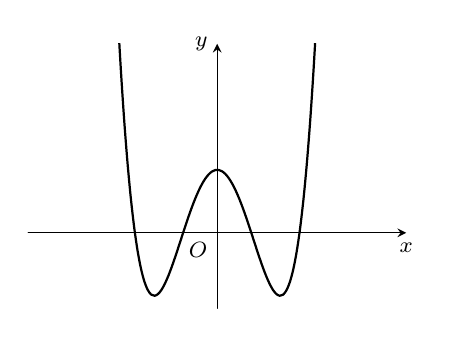
\begin{tikzpicture}[scale=0.8, font=\footnotesize, line join=round, line cap=round, >=stealth]
		\def\a{2} %Hệ số a phải khác 0
		\def\b{-4}
		\def\c{1}
		\draw[->] (-3,0) -- (3,0) node[below] { $x$};
		\draw[->] (0,-1.2) -- (0,3) node[left] { $y$};
		\draw (0,0)node[below left]{$O$};
\begin{scope}
		\clip (-3,-1.2)rectangle(3,3);
		\draw[thick,samples=150,smooth,domain=-4:4] plot(\x,{\a*(\x)^4+(\b)*(\x)^2+(\c)});
\end{scope}
\end{tikzpicture}}
	\loigiai{
		Từ hình dạng của đồ thị, ta có $a>0$.\\ 
		Đồ thị hàm số có $3$ điểm cực trị nên $ab<0 \Rightarrow b<0$ (vì $a>0$).\\
		Vì giao điểm của đồ thị và trục tung nằm phía trên trục hoành nên $c>0$.\\
		Vậy $a>0$, $b<0$, $c>0$.
	}
\end{ex}

\begin{ex}%[Kiểm tra chuyên đề lần 2, THPT Chuyên Vĩnh Phúc Lần 2, 2023]%[Đăng Tạ, 12EX6]%[2D2B6-1]
	Tìm tất cả các giá trị của $a$ thỏa mãn $(a-1)^{-\frac{2}{3}}<(a-1)^{-\frac{1}{3}}$.
	\choice
	{$1<a<2$}
	{$a>1$}
	{\True $a>2$}
	{$0<a<1$}
	\loigiai{
		Ta có $-\dfrac{2}{3}<-\dfrac{1}{3}$, kết hợp với $(a-1)^{-\frac{2}{3}}<(a-1)^{-\frac{1}{3}}$. Suy ra hàm số $y=(a-1)^x$ đồng biến.\\
		Vậy $a-1>1 \Leftrightarrow a>2$.
	}
\end{ex}

\begin{ex}%[Kiểm tra chuyên đề lần 2, THPT Chuyên Vĩnh Phúc Lần 2, 2023]%[Đăng Tạ, 12EX6]%[2D2B6-1]
	Tìm tất cả các giá trị của $x$ thỏa mãn $\left(\tan \dfrac{\pi}{7}\right)^{x^2-x-9} \leq \left(\tan \dfrac{\pi}{7}\right)^{x-1}$.
	\choice
	{$x \leq -2$}
	{$x\geq 4$}
	{$-2\leq x\leq 4$}
	{\True $x\leq -2$; $x \geq 4$}
	\loigiai{
		Vì $0< \tan \dfrac{\pi}{7} <1$ nên ta có 
\begin{eqnarray*}
			& & \left(\tan \dfrac{\pi}{7}\right)^{x^2-x-9} \leq \left(\tan \dfrac{\pi}{7}\right)^{x-1}\\
			&\Leftrightarrow & x^2-x-9 \geq x-1\\
			&\Leftrightarrow & x^2-2x-8 \geq 0\\
			&\Leftrightarrow & \hoac{&x\leq -2\\&x \geq 4.}
\end{eqnarray*} 
	}
\end{ex}

\begin{ex}%[Kiểm tra chuyên đề lần 2, THPT Chuyên Vĩnh Phúc Lần 2, 2023]%[Đăng Tạ, 12EX6]%[2D2B4-2]
	Cho hàm số $y=x\cdot \mathrm{e}^{-x}$. Mệnh đề nào sau đây đúng?
	\choice
	{$x\cdot y'= (1+x)y$}
	{$(1-x)y'=x\cdot y$}
	{$(1+x)\cdot y'=(x-1)\cdot y$}
	{\True $x\cdot y'=(1-x)\cdot y$}
	\loigiai{
		Ta có $y'= \mathrm{e}^{-x} \left(1-x\right)$.\\
		Lại có $(1-x)\cdot y =(1-x) \cdot x \cdot \mathrm{e}^{-x} =x\cdot \mathrm{e}^{-x} \left(1-x\right) = x\cdot y'$.\\
		Vậy $x\cdot y'=(1-x)\cdot y$.
	}
\end{ex}

\begin{ex}%[Kiểm tra chuyên đề lần 2, THPT Chuyên Vĩnh Phúc Lần 2, 2023]%[Đăng Tạ, 12EX6]%[2D2B5-4]
	Tìm tập nghiệm $S$ của phương trình $\log_2 \left(9-2^x\right)=3-x$.
	\choice
	{$S=\{1;3\}$}
	{$S=\{-3;1\}$}
	{\True $S=\{0;3\}$}
	{$S=\{-3;0\}$}
	\loigiai{
		ĐKXĐ $9-2^x > 0$.\\
		Phương trình đã cho tương đương với phương trình 
\begin{eqnarray*}
			& & 9-2^x=2^{3-x}\\
			&\Leftrightarrow & 9-2^x=\dfrac{8}{2^x}\\
			&\Leftrightarrow & 2^{2x}-9\cdot 2^x+8=0\\
			&\Leftrightarrow &  \hoac{&2^x=1\\&2^x=8}\\
			&\Leftrightarrow & \hoac{&x=0\text{ (thỏa điều kiện)}\\&x=3\text{ (thỏa điều kiện).}}
\end{eqnarray*}
		Vậy tập nghiệm của phương trình đã cho là $S=\{0;3\}$.
	}
\end{ex}

\begin{ex}%[Kiểm tra chuyên đề lần 2, THPT Chuyên Vĩnh Phúc Lần 2, 2023]%[Đăng Tạ, 12EX6]%[2D2B3-2]
	Cho $a$, $b$ là các số thực dương và $a\neq 1$. Khẳng định nào sau đây đúng?
	\choice
	{$\log_{\sqrt{a}} \left(a^2+ab\right) = 4+2\log_a b$}
	{$\log_{\sqrt{a}} \left(a^2+ab\right) = 4\log_a (a+b)$}
	{\True $\log_{\sqrt{a}} \left(a^2+ab\right) = 2+2\log_a (a+b)$}
	{$\log_{\sqrt{a}} \left(a^2+ab\right) = 1+4\log_a b$}
	\loigiai{
		Ta có $\log_{\sqrt{a}} \left(a^2+ab\right) = 2 \log_a [a\left(a+b\right)] = 2\left[\log_a a + \log_a (a+b)\right]= 2 + 2\log_a (a+b)$.
	}
\end{ex}

\begin{ex}%[Kiểm tra chuyên đề lần 2, THPT Chuyên Vĩnh Phúc Lần 2, 2023]%[Đăng Tạ, 12EX6]%[2D1B2-2] 
	Cho hàm số $y=f(x)$ liên tục trên $\mathbb{R}$ với bảng xét dấu đạo hàm như sau
\begin{center}

\begin{tikzpicture}
		\tkzTabInit[nocadre=false,lgt=1.2,espcl=2.5,deltacl=0.6]
		{$x$ /0.6, $y'$ /0.6}
		{-$\infty$,$-3$,$1$,$2$,$+\infty$}
		\tkzTabLine{,-,$0$,+,$0$,+,$0$,-,}
\end{tikzpicture}
\end{center}
	Hỏi hàm số $y=f(x)$ có bao nhiêu điểm cực trị?
	\choice
	{$3$}
	{$1$}
	{$0$}
	{\True $2$}
	\loigiai{
		Từ bảng xét dấu, ta có $y'$ đổi dấu khi đi qua $x=-3$, $x=2$ nên hàm số $y=f(x)$ có hai điểm cực trị.
	}
\end{ex}

\begin{ex}%[Kiểm tra chuyên đề lần 2, THPT Chuyên Vĩnh Phúc Lần 2, 2023]%[Đăng Tạ, 12EX6]%[2H3B1-3]
	Trong KG $Oxyz$, mặt cầu tâm $I(2;-3;1)$ và đi qua điểm $A(6;1;3)$ có phương trình là
	\choice
	{$x^2+y^2+z^2+4x-6y+2z-22=0$}
	{\True $x^2+y^2+z^2-4x+6y-2z-22=0$}
	{$x^2+y^2+z^2+12x+2y+6z-10=0$}
	{$x^2+y^2+z^2-12x-2y-6z-10=0$}
	\loigiai{
		Ta có $R=IA=\sqrt{4^2+4^2+2^2}=6$.\\
		Phương trình mặt cầu tâm $I(2;-3;1)$ và $R=6$ có dạng
\begin{center}
			$(x-2)^2+(x+3)^2+(x-1)^2=6^2\Leftrightarrow x^2+y^2+z^2-4x+6y-2z-22=0$.
\end{center}	
	}
\end{ex}

\begin{ex}%[Kiểm tra chuyên đề lần 2, THPT Chuyên Vĩnh Phúc Lần 2, 2023]%[Đăng Tạ, 12EX6]%[2D2B4-1]
	Tìm tập xác định $\mathscr{D}$ của hàm số $y=\dfrac{\mathrm{e}^x}{\mathrm{e}^x-1}$.
	\choice
	{$\mathscr{D}=\mathbb{R}$}
	{$\mathscr{D}=\mathbb{R}\setminus \{\mathrm{e}\}$}
	{$\mathscr{D}=\mathbb{R}\setminus \{1\}$}
	{\True $\mathscr{D}=\mathbb{R}\setminus \{0\}$}
	\loigiai{
		Điều kiện $\mathrm{e}^x-1\neq 0\Leftrightarrow x\neq 0$.\\
		Vậy tập xác định của hàm số là $\mathscr{D}=\mathbb{R}\setminus \{0\}$.
	}
\end{ex}

\begin{ex}%[Kiểm tra chuyên đề lần 2, THPT Chuyên Vĩnh Phúc Lần 2, 2023]%[Đăng Tạ, 12EX6]%[2D3B1-2] 
	Cho nguyên hàm $I=\displaystyle\int\limits x^2\sqrt{4-x^2}\mathrm{\,d}x$. Nếu đặt $x=2\sin t$ với $t\in \left[-\dfrac{\pi}{2};\dfrac{\pi}{2}\right]$ thì
	\choice
	{$I=2t+\dfrac{\cos 4t}{2}+C$}
	{$I=2t+\dfrac{\sin 8t}{4}+C$}
	{$I=2t-\dfrac{\cos 4t}{2}+C$}
	{\True $I=2t-\dfrac{\sin 4t}{2}+C$}
	\loigiai{
		Ta có $x=2\sin t \Rightarrow \mathrm{\,d}x=2\cos t\mathrm{\,d}t$. Khi đó
\begin{eqnarray*}
			I&=&\displaystyle\int\limits x^2\sqrt{4-x^2}\mathrm{\,d}x\\
			&=&\displaystyle\int\limits 4\sin ^2t\sqrt{4-4\sin ^2t}\cdot 2\cos t\mathrm{\,d}t\\
			&=&\displaystyle\int\limits 4\sin ^2t\cdot 2\cos t \cdot 2\cos t\mathrm{\,d}t\\
			&=&\displaystyle\int\limits 4\sin^2 2t\mathrm{\,d}t=\displaystyle\int\limits 2\cdot (1-\cos 4t)\mathrm{\,d}t\\
			&=& 2t-\dfrac{\sin 4t}{2}+C.
\end{eqnarray*}
	}
\end{ex}

\begin{ex}%[Kiểm tra chuyên đề lần 2, THPT Chuyên Vĩnh Phúc Lần 2, 2023]%[Đăng Tạ, 12EX6]%[1H3B4-3]
	Cho hình chóp $S.ABCD$ có đáy $ABCD$ là hình vuông cạnh $a$, cạnh $SA=a$ và vuông góc với mặt phẳng đáy. Góc giữa hai mặt phẳng $(SBC)$ và $(ABCD)$ bằng
	\choice
	{$90^\circ$}
	{$30^\circ$}
	{$60^\circ$}
	{\True $45^\circ$}
	\loigiai{
		\immini{
			Ta có $\heva{&BC \text{ chung}\\& \text{Trong } (ABCD) \colon BC \perp AB\\& \text{Trong } (SAB) \colon BC \perp SB}$.\\
			Suy ra $\left((SBC),(ABCD)\right) = \left(AB,SB\right)=\widehat{SBA}$.\\
			Ta có $\tan \widehat{SBA}=\dfrac{SA}{AB}=\dfrac{a}{a}=1\Rightarrow \widehat{SBA}=45^\circ$.
		}{
\begin{tikzpicture}[scale=0.8,>=stealth, font=\footnotesize, line join=round, line cap=round]
			\def\a{4}
			\def\h{4}
			\path 	(0:0) coordinate (A)
			++(0:\a) coordinate (D)
			++(-130:\a/2) coordinate (C)
			($(A)+(C)-(D)$) coordinate (B)
			($(A)+(90:\h)$) coordinate (S)
			(intersection of A--C and B--D) coordinate (O);%giao điểm O
			\draw[dashed,thick] 	(B)--(A)--(D)	(A)--(S);
			\draw[thick] 			(B)-- (C)--(D)
			(B)--(S)	(C)--(S)	(D)--(S);
			\foreach \x/\g in {A/135,B/-135,C/-45,D/45,S/90}
			\fill[black] 	(\x) circle (1.5pt)
			($(\g:3mm)+(\x)$) node {$\x$};	
			\tkzMarkAngles[size=1,arc=ll,mark=|](A,B,S)
\end{tikzpicture}
		}
	}
\end{ex}

\begin{ex}%[Kiểm tra chuyên đề lần 2, THPT Chuyên Vĩnh Phúc Lần 2, 2023]%[Đăng Tạ, 12EX6]%[2D1B4-2] 
	Cho hàm số $y=\dfrac{x-1}{\sqrt{x^2+2(m-1)x+m^2}}$ với $m$ là tham số thực và $m>\dfrac{1}{2}$. Hỏi đồ thị của hàm số có bao nguyên đường tiệm cận?
	\choice
	{$3$}
	{$1$}
	{$4$}
	{\True $2$}
	\loigiai{
		Ta có $x^2+2(m-1)x+m^2 =x^2+2(m-1)x+(m-1)^2+2m-1 = (x-m+1)^2+2m-1>0$ với $m>\dfrac{1}{2}$.\\
		Do đó, hàm số có tập xác định là $\mathscr{D}=\mathbb{R}$.\\
		Vì $\lim\limits_{x\to +\infty} \dfrac{x-1}{\sqrt{x^2+2(m-1)x+m^2}}=1$ nên $y=1$ là tiệm cận ngang của đồ thị hàm số.\\
		Vì $\lim\limits_{x\to -\infty} \dfrac{x-1}{\sqrt{x^2+2(m-1)x+m^2}}=-1$ nên $y=-1$ là tiệm cận ngang của đồ thị hàm số.\\
		Vậy đồ thị hàm số có hai đường tiệm cận.
	}
\end{ex}

\begin{ex}%[Kiểm tra chuyên đề lần 2, THPT Chuyên Vĩnh Phúc Lần 2, 2023]%[Đăng Tạ, 12EX6]%[2D2B5-1]
	Tính $P$ là tổng bình phương tất cả các nghiệm của phương trình $2^{x-1}+2^{2-x}=3$.
	\choice
	{$P=1$}
	{$P=3$}
	{\True $P=5$}
	{$P=9$}
	\loigiai{
	Ta có	
\begin{eqnarray*}
			&& 2^{x-1}+2^{2-x}=3\\
			&\Leftrightarrow & \dfrac{1}{2}\cdot 2^x+\dfrac{4}{2^x}=3\\
			&\Leftrightarrow & \dfrac{1}{2}\cdot 2^{2x}-3\cdot 2^x+4=0\\
			&\Leftrightarrow & \hoac{&2^x=2 \\&2^x=4}\\
			&\Leftrightarrow & \hoac{&x=1 \\&x=2.}
\end{eqnarray*}
	Vậy $P=1^2+2^2=5$.
	}
\end{ex}

\begin{ex}%[Kiểm tra chuyên đề lần 2, THPT Chuyên Vĩnh Phúc Lần 2, 2023]%[Đăng Tạ, 12EX6]%[2D1B3-1]
	Hàm số nào sau đây không có giá trị nhỏ nhất và giá trị lớn nhất trên đoạn $[-2;2]$?
	\choice
	{$y=x^4+x^2$}
	{$y=x^3+2$}
	{\True $y=\dfrac{x-1}{x+1}$}
	{$y=-x+1$}
	\loigiai{
		Xét hàm số $y=\dfrac{x-1}{x+1}$ có tập xác định $\mathscr{D} = \mathbb{R} \setminus \{-1\}$.\\
		Vì $\lim\limits_{x \rightarrow (-1)^+}=-\infty$; $\lim\limits_{x \rightarrow (-1)^-}=+\infty$ nên hàm số này không có giá trị lớn nhất và giá trị nhỏ nhất trên đoạn $[-2;2]$.
	}
\end{ex}

\begin{ex}%[Kiểm tra chuyên đề lần 2, THPT Chuyên Vĩnh Phúc Lần 2, 2023]%[Đăng Tạ, 12EX6]%[2D1B2-1]
	Biết rằng hàm số $y=x^3+4x^2-3x+7$ đạt cực tiểu tại $x_\text{CT}$. Mệnh đề nào sau đây là đúng?
	\choice
	{\True $x_\text{CT}=\dfrac{1}{3}$}
	{$x_\text{CT}=-\dfrac{1}{3}$}
	{$x_\text{CT}=1$}
	{$x_\text{CT}=-3$}
	\loigiai{
		Ta có $y=x^3+4x^2-3x+7 \Rightarrow y'=3x^2+8x-3$. Cho $y'=0 \Leftrightarrow 3x^2+8x-3=0 \Leftrightarrow \hoac{&x=-3\\&x=\dfrac{1}{3}.}$\\
		Bảng xét dấu đạo hàm
\begin{center}

\begin{tikzpicture}
			\tkzTabInit[nocadre=false,lgt=1.2,espcl=3,deltacl=0.6]
			{$x$ /0.8, $y'$ /0.8}
			{$-\infty$,$-3$,$\dfrac{1}{3}$,$+\infty$}
			\tkzTabLine{ ,+,0,-,0,+, }
\end{tikzpicture}
\end{center}
		Từ bảng xét dấu đạo hàm ta có $x_\text{CT}=\dfrac{1}{3}$.
	}
\end{ex}

\begin{ex}%[Kiểm tra chuyên đề lần 2, THPT Chuyên Vĩnh Phúc Lần 2, 2023]%[Đăng Tạ, 12EX6]%[2D2B3-2]
	Cho $a$, $b$, $c$ là các số thực dương khác $1$ và thỏa $\log_a b^2 = x$, $\log_{b^2} \sqrt{c} =y$. Tính giá trị của biểu thức $P=\log_c a$.
	\choice
	{$P=\dfrac{xy}{2}$}
	{$P=2xy$}
	{\True $P=\dfrac{1}{2xy}$}
	{$P=\dfrac{2}{xy}$}
	\loigiai{
		Ta có $x=\log_a b^2 = 2\log_a b \Leftrightarrow \log_a b =\dfrac{x}{2}$ và $y=\log_{b^2} \sqrt{c} = \dfrac{1}{4}\log_b c \Rightarrow \log_b c = 4y$. Do đó\\
		$$P=\log_c a= \dfrac{\log_b a}{\log_b c} = \dfrac{1}{\log_a b\cdot \log_b c}  = \dfrac{1}{2xy}.$$
	}
\end{ex}

\begin{ex}%[Kiểm tra chuyên đề lần 2, THPT Chuyên Vĩnh Phúc Lần 2, 2023]%[Đăng Tạ, 12EX6]%[2H1B1-2]
	Khẳng định nào sau đây là khẳng định \textbf{sai}?
	\choice
	{Mỗi cạnh của khối đa diện là cạnh chung của đúng $2$ mặt của khối đa diện}
	{\True Hai mặt bất kì của khối đa diện luôn có ít nhất một điểm chung}
	{Mỗi đỉnh của khối đa diện là đỉnh chung của ít nhất $3$ mặt}
	{Mỗi mặt của khối đa diện có ít nhất ba cạnh}
	\loigiai{
		Hai mặt bất kì của khối đa diện chỉ có thể hoặc không có điểm chung, hoặc chỉ có một đỉnh chung, hoặc chỉ có một cạnh chung.
	}
\end{ex}

\begin{ex}%[Kiểm tra chuyên đề lần 2, THPT Chuyên Vĩnh Phúc Lần 2, 2023]%[Đăng Tạ, 12EX6]%[2D2B2-1]
	Tìm tập xác định $\mathscr{D}$ của hàm số $y=\left(x^4-3x^2-4\right)^{\sqrt{2}}$.
	\choice
	{\True $\mathscr{D}=(-\infty;-2)\cup (2;+\infty)$}
	{$\mathscr{D}=(-\infty;+\infty)$}
	{$\mathscr{D}=(-\infty;-1)\cup (4;+\infty)$}
	{$\mathscr{D}=(-\infty;-2]\cup [2;+\infty)$}
	\loigiai{
		Điều kiện $x^4-3x^2-4>0 \Leftrightarrow \left(x^2+1\right)\left(x^2-4\right)>0 \Leftrightarrow x^2>4 \Leftrightarrow \hoac{&x>2\\&x<-2.}$\\
		Vậy tập xác định của hàm số là $\mathscr{D}=(-\infty;-2)\cup (2;+\infty)$.
	}
\end{ex}

\begin{ex}%[Kiểm tra chuyên đề lần 2, THPT Chuyên Vĩnh Phúc Lần 2, 2023]%[Đăng Tạ, 12EX6]%[2D2B4-2]
	Tính đạo hàm của hàm số $y=\log 2x$.
	\choice
	{$y'=\dfrac{1}{x \ln 2}$}
	{\True $y'=\dfrac{1}{x \ln 10}$}
	{$y'=\dfrac{1}{2 x \ln 10}$}
	{$y'=\dfrac{\ln 10}{x}$}
	\loigiai{
		Với $x>0$ ta có	$ y'= \dfrac{(2x)'}{2x \ln 10} = \dfrac{1}{x \ln 10}$.
	}
\end{ex}

\begin{ex}%[Kiểm tra chuyên đề lần 2, THPT Chuyên Vĩnh Phúc Lần 2, 2023]%[Đăng Tạ, 12EX6]%[2D1B5-1] 
	\immini{	Đường cong trong hình bên là đồ thị của hàm số nào?
		\choice
		{ $y=-x^3+1$}
		{\True $y=-x^3+2$}
		{$y=-x^3+3 x+2$}
		{$y=-x^3+3 x^2-3 x+2$} 
	}{
\begin{tikzpicture}[>=stealth,line join=round,line cap=round,font=\footnotesize,scale=0.7]
		\draw[->] (0,-2)--(0,5)node[right]{$y$};
		\draw[->] (-1.8,0)--(2,0)node[below]{$x$};
		\fill (0,0)node[below left]{ $O$}circle(1.2pt);	
		\draw[smooth,samples=300,domain=-1.3:1.5] plot(\x,{-(\x)^3+2});
		\draw[fill=black] (0,2) circle(1pt) node [shift={(30:.2)}] {$2$};
\end{tikzpicture} 
	}
	\loigiai{
		Dựa vào hình vẽ ta thấy đây là đồ thị hàm bậc ba với hệ số $a<0$.\\
		Đồ thị cắt trục $Oy$ tại điểm có tung độ $y=2$ nên loại $y=-x^3+1$.\\
		Đồ thị hàm số không có cực trị và $y=-x^3+2$ có $y'=-3x^2 \leq 0$ nên chọn.
	}
\end{ex}

\begin{ex}%[Kiểm tra chuyên đề lần 2, THPT Chuyên Vĩnh Phúc Lần 2, 2023]%[Đăng Tạ, 12EX6]%[2D1B1-2] 
	Cho hàm số $y=2 x^4-4x^2$. Mệnh đề nào sau đây \textbf{sai}?
	\choice
	{\True Hàm số đã cho đồng biến trên các khoảng $(-\infty;-1)$ và $(1;+ \infty)$}
	{Trên các khoảng $(-1; 0)$ và $(1;+\infty)$, $y'>0$ nên hàm số đã cho đồng biến}
	{Trên các khoảng $(-\infty;-1)$ và $(0; 1)$, $y'<0$ nên hàm số đã cho nghịch biến}
	{Hàm số đã cho nghịch biến trên các khoảng $(-\infty;-1)$ và $(0; 1)$}
	\loigiai{
		Ta có $y'=0 \Leftrightarrow 8x^3-8x =0 \Leftrightarrow \hoac{&x=0\\&x= \pm 1.}$\\
		Bảng biến thiên
\begin{center}

\begin{tikzpicture}
			\tkzTabInit[nocadre=false,lgt=1.2,espcl=2.5,deltacl=0.6]
			{$x$ /0.6, $y'$ /0.6, $y$ /1.5}
			{-$\infty$,$-1$,$0$,$1$,$+\infty$}
			\tkzTabLine{,-,$0$,+,$0$,-,$0$,+,}
			\tkzTabVar{+/$+\infty$,-/$-2$,+/$0$,-/$-2$,+/$+\infty$}
\end{tikzpicture}
\end{center}
		Dựa vào bảng biến thiên ta chọn đáp án: Hàm số đã cho đồng biến trên các khoảng $(-\infty;-1)$ và $(1;+ \infty)$.
	}
\end{ex}

\begin{ex}%[Kiểm tra chuyên đề lần 2, THPT Chuyên Vĩnh Phúc Lần 2, 2023]%[Đăng Tạ, 12EX6]%[2H1B3-2]
	Cho hình lăng trụ tam giác $ABC. A'B'C'$. Gọi $M$, $N$ lần lượt là trung điểm của $BB'$, $CC'$. Mặt phẳng $\left(A'MN\right)$ chia khối lăng trụ thành hai phần, đặt $V_1$ là thể tích của phần đa diện chứa điểm $B$, $V_2$ là thể tích phần còn lại. Tính tỉ số $\dfrac{V_1}{V_2}$.
	\choice
	{\True $\dfrac{V_1}{V_2}=2$}
	{$\dfrac{V_1}{V_2}=3$}
	{ $\dfrac{V_1}{V_2}=\dfrac{7}{2}$}
	{$\dfrac{V_1}{V_2}=\dfrac{5}{2}$}
	\loigiai{
		\immini{	
			Gọi $V$ là thể tích hình lăng trụ tam giác $ABC. A'B'C'$ và $P$ là trung điểm của $AA'$. Khi đó \\
			$V_2=V_{A'B'C'.PMN}-V_{A'.PMN}=\dfrac{V}{2}-\dfrac{V}{6}=\dfrac{V}{3}$.\\
			Suy ra $V_1=V-V_2=\dfrac{2V}{3}$. Do đó $\dfrac{V_1}{V_2}=2$.}{
\begin{tikzpicture}[scale=1, font=\footnotesize, line join=round, line cap=round, >=stealth,scale=0.8]
			\def\a{1}%qua
			\def\b{3}%cao
			\coordinate (A) at (0,0);
			\coordinate (B) at (4,0);
			\coordinate (C) at (1.5,-1);
			\coordinate (A') at ($(A)+(\a,\b)$);
			\coordinate (B') at ($(B)+(\a,\b)$);
			\coordinate (C') at ($(C)+(\a,\b)$);
			\coordinate (M) at ($(B)!0.5!(B')$);
			\coordinate (N) at ($(C)!0.5!(C')$);
			\coordinate (P) at ($(A)!0.5!(A')$);
			\draw (M)--(N)--(A')--(A)--(C)--(B)--(B')--(A')--(C')--(C) (B')--(C') (N)--(P);
			\draw[dashed] (A)--(B) (M)--(A') (P)--(M);
			\foreach \p/\g in {A/180, B/0, C/-90, A'/90, B'/90, C'/-45, M/0, N/-30, P/180}
			\draw[fill=black] (\p) circle(1pt) node [shift={(\g:.3)}] {$\p$};
\end{tikzpicture}		
		}
	}
\end{ex}

\begin{ex}%[Kiểm tra chuyên đề lần 2, THPT Chuyên Vĩnh Phúc Lần 2, 2023]%[Đăng Tạ, 12EX6]%[2D2B5-1] 
	Số nghiệm của phương trình $\dfrac{x^3-5x^2+6 x}{\ln (x-1)}=0$ là
	\choice
	{$0$}
	{\True $1$}
	{$2$}
	{$3$}
	\loigiai{
		Điều kiện $\heva{&x-1>0\\&\ln (x-1) \neq 0} \Leftrightarrow \heva{&x>1\\&x \neq 2}$. Khi đó\\
		$$\dfrac{x^3-5x^2+6 x}{\ln (x-1)}=0 \Rightarrow x^3-5x^2+6 x =0 \Leftrightarrow \hoac{&x=0\\&x=2\\&x=3.}$$\\
		Kết hợp với điều kiện ta được $x=3$.
	}
\end{ex}

\begin{ex}%[Kiểm tra chuyên đề lần 2, THPT Chuyên Vĩnh Phúc Lần 2, 2023]%[Đăng Tạ, 12EX6]%[2D2B5-1]
	Có tất cả bao nhiêu số nguyên thỏa mãn bất phương trình $\log_{\frac{1}{2}}\left[\log_2 (2-x)^2\right]>0$?
	\choice
	{$1$}
	{$2$}
	{$3$}
	{\True $0$}
	\loigiai{
		Điều kiện $\heva{&\log_2 (2-x)^2>0\\ &(2-x)^2>0}\Leftrightarrow \heva{&\hoac{x<1\\x>3}\\&x\neq 2}\Leftrightarrow \hoac{x<1\\x>3}$. Khi đó ta có \\
\begin{eqnarray*}
			&&\log_{\frac{1}{2}}\left[\log_2 (2-x)^2\right]>0\\
			&\Leftrightarrow & \log_2 (2-x)^2<1\\
			&\Leftrightarrow & (2-x)^2<2\\
			&\Leftrightarrow & 2-\sqrt{2}<x<2+\sqrt{2}.
\end{eqnarray*}
		Kết hợp với điều kiện, bất phương trình có nghiệm $x\in (2-\sqrt{2};1)\cup (3;2+\sqrt{3})$.\\
		Mà $x\in \mathbb{Z} \Rightarrow x\in \varnothing$.\\
		Vậy bất phương trình không có nghiệm nguyên.
	}
\end{ex}

\begin{ex}%[Kiểm tra chuyên đề lần 2, THPT Chuyên Vĩnh Phúc Lần 2, 2023]%[Đăng Tạ, 12EX6]%[2D2K4-4] 
	Xét các số thực dương $x$, $y$ thỏa mãn $\log _{\tfrac{1}{2}} x+\log _{\tfrac{1}{2}} y \leq \log _{\tfrac{1}{2}}\left(x+y^2\right)$. Tìm giá trị nhỏ nhất của biểu thức $P=x+3y$.
	\choice
	{\True $P_{\min }=9$}
	{$P_{\min }=8$}
	{$P_{\min }=\dfrac{17}{2}$}
	{$P_{\min }=\dfrac{25 \sqrt{2}}{4}$}
	\loigiai{
		Ta có $\log _{\tfrac{1}{2}} x+\log _{\tfrac{1}{2}} y \leq \log _{\tfrac{1}{2}}\left(x+y^2\right) \Leftrightarrow \log _{\tfrac{1}{2}} xy \leq \log _{\tfrac{1}{2}}\left(x+y^2\right) \Leftrightarrow xy \geq x+y^2 \Leftrightarrow x(y-1)\geq y^2. \quad (1)$ \\
		Do $y\leq 1$ không thỏa mãn $(1)$ nên $y>1$. Từ
		$(1)\Rightarrow x \geq \dfrac{y^2}{y-1}$. Khi đó
		$$P=x+3y \geq \dfrac{y^2}{y-1}+3y =y+1+\dfrac{1}{y-1}+3y= \dfrac{1}{y-1}+4(y-1)+5 \geq 2\sqrt{ \dfrac{1}{y-1}\cdot 4(y-1)}+5=9.$$
		Vậy $P_{\min }=9$ khi $x=\dfrac{9}{2}$, $y=\dfrac{3}{2}$.
	}
\end{ex}

\begin{ex}%[Kiểm tra chuyên đề lần 2, THPT Chuyên Vĩnh Phúc Lần 2, 2023]%[Đăng Tạ, 12EX6]%[2D1K5-4]
	Tìm tổng tất cả các giá trị thực của tham số $m$ để đường thẳng $d \colon y=2x + m$ cắt đồ thị hàm số $(C) \colon y=\dfrac{2x-4}{x-1}$ tại hai điểm phân biệt $A$ và $B$ sao cho $4S_{\triangle IAB}=15$, với $I$ là giao điểm của hai đường tiệm cận của đồ thị.
	\choice
	{\True $0$}
	{$15$}
	{$10$}
	{$8$}
	\loigiai{
		Tập xác định $\mathscr{D} =\mathbb{R} \setminus \{1\}$.\\
		Ta có $\lim\limits_{x \rightarrow 1^+} \dfrac{2x-4}{x-1} = -\infty$; $\lim\limits_{x \rightarrow 1^-} \dfrac{2x-4}{x-1} = +\infty \Rightarrow (C)$ có tiệm cận đứng $x=1$.\\
		Lại có $\lim\limits_{x \rightarrow \pm\infty} \dfrac{2x-4}{x-1} = 2 \Rightarrow (C)$ có tiệm cận ngang $y=2$.\\
		Vì $I$ là giao điểm của hai đường tiệm cận của đồ thị $\Rightarrow I(1;2)$.\\
		Phương trình hoành độ giao điểm của $(C)$ và $(d)$ là
		\begin{eqnarray*}
			& & \dfrac{2x-4}{x-1} = 2x+m\\
			&\Leftrightarrow & 2x-4=(2x+m)\cdot (x-1)\\
			&\Leftrightarrow & 2x-4=2x^2-2x+mx-m\\
			&\Leftrightarrow & 2x^2+(m-4)x + (4-m)=0 \quad (1)
		\end{eqnarray*}
		Đường thẳng $(d)$ cắt $(C)$ tại hai điểm phân biệt $\Leftrightarrow$ Phương trình $(1)$ có hai nghiệm phân biệt khác $1$. Do đó
		\begin{eqnarray*}
			&&\heva{&\Delta > 0 \\ & 2\cdot 1^2 +(m-4)\cdot 1 +4-m \neq 0} \\
			&\Leftrightarrow &\heva{&(m-4)^2-4\cdot 2 \cdot (4-m)>0\\& 2 \neq 0 \text{ (luôn đúng)}} \\
			&\Leftrightarrow & m^2 - 16>0 \\
			&\Leftrightarrow & \hoac{&m<-4\\&m>4.}
		\end{eqnarray*}
		Khi đó, $(1)$ có hai nghiệm phân biệt $x_1$, $x_2$ thỏa $\heva{&x_1+x_2=\dfrac{4-m}{2}\\&x_1\cdot x_2=\dfrac{4-m}{2}}$.\\
		Tọa độ hai giao điểm là $A(x_1;2x_1+m)$, $B(x_2;2x_2+m)$.
		\begin{eqnarray*}
			&AB & =\sqrt{\left(x_2-x_1\right)^2+\left(2x_2-2x_1\right)^2}\\
			& & =\sqrt{5} \cdot \sqrt{\left(x_1-x_2\right)^2}\\
			& & =\sqrt{5} \cdot \sqrt{\left(x_1+x_2\right)^2-4x_1x_2}\\
			& & =\sqrt{5} \cdot \sqrt{\left(\dfrac{4-m}{2}\right)^2-4\cdot \dfrac{4-m}{2}}\\
			& & =\dfrac{\sqrt{5}}{2}\cdot \sqrt{m^2-8m+16-32+8m}\\
			& & =\dfrac{\sqrt{5}}{2}\cdot \sqrt{m^2-16}.
		\end{eqnarray*}
		Ta có $(d) \colon y=2x+m \Leftrightarrow 2x-y+m=0$.\\
		$\Rightarrow \mathrm{d} (I;d) = \dfrac{|2\cdot 1-2+m|}{\sqrt{2^2+1^2}} = \dfrac{|m|}{\sqrt{5}}$.\\
		Ta có
		\begin{eqnarray*}
			& & 4S_{\triangle IAB}=15\\
			&\Leftrightarrow & 4\cdot \dfrac{1}{2} \cdot \mathrm{d}(I;d)\cdot AB =15\\
			&\Leftrightarrow & 4\cdot \dfrac{1}{2} \cdot \dfrac{|m|}{\sqrt{5}} \cdot \sqrt{m^2-16} = 15\\
			&\Leftrightarrow & m^4-16m^2-225=0\\
			&\Leftrightarrow & \hoac{&m^2=-9\\&m^2=25}\\
			&\Leftrightarrow & m=\pm 5 \text{\quad (thỏa mãn).}
		\end{eqnarray*}
		Tổng các giá trị thực của tham số $m$ là $-5+5=0$.
	}
\end{ex}

\begin{ex}%[Kiểm tra chuyên đề lần 2, THPT Chuyên Vĩnh Phúc Lần 2, 2023]%[Đăng Tạ, 12EX6]%[2D1K2-4]
	Cho hàm số $y=x^3-3mx^2+3\left(m^2-1\right)x-m^3$ với $m$ là tham số thực. Gọi $S$ là tập hợp tất cả các giá trị của $m$ sao cho đồ thị hàm số có hai điểm cực trị. Biết rằng khi $m$ thay đổi trong $S$, các điểm cực đại của đồ thị hàm số cũng thay đổi nhưng luôn nằm trên một đường thẳng $d$ cố định. Hỏi $d$ song song với	đường thẳng nào sau đây?
	\choice
	{$y=-2x$}
	{\True $y=-3x+5$}
	{$y=2x+4$}
	{$y=-3x-1$}
	\loigiai{
		Ta có $y=x^3-3mx^2+3\left(m^2-1\right)x-m^3\Rightarrow y'=3x^2-6mx+3\left(m^2-1\right)$.\\
		Cho $y'=0 \Leftrightarrow x^2-2mx+\left(m^2-1\right) =0 \Leftrightarrow (x-m)^2=1 \Leftrightarrow \hoac{&x=m+1\\&x=m-1.}$\\
		Phương trình $y'=0$ luôn có hai nghiệm phân biệt là $m+1$ và $m-1$ nên đồ thị hàm số luôn có hai điểm cực trị.\\
		Ta có bảng biến thiên
		\begin{center}
			
\begin{tikzpicture}
			\tkzTabInit[nocadre=false,lgt=1.2,espcl=3,deltacl=0.6]
			{$x$ /0.8, $y'$ /0.8, $y$ /1.5}
			{$-\infty$,$m-1$,$m+1$,$+\infty$}
			\tkzTabLine{ ,+,0,-,0,+, }
			\tkzTabVar{-/$-\infty$,+/$y(m-1)$,-/$y(m+1)$,+/$+\infty$}
			\end{tikzpicture}
		\end{center}
		Từ bảng biến thiên ta có hàm số đạt cực đại tại $x_\text{CĐ}=m-1$.\\
		Khi đó, $y_\text{CĐ} = (m-1)^3-3m(m-1)^2 +3\left(m^2-1\right)(m-1)-m^3 = -3m+2$.\\
		Vậy điểm cực đại của đồ thị hàm số có tọa độ $(m-1;-3m+2) = (m-1;-3(m-1)-1)$.\\
		Do đó đường thẳng cố định luôn đi qua điểm cực đại của đồ thị hàm số là $d \colon y=-3x-1$.\\
		Vậy $d$ song song với đường thẳng $y=-3x+5$.
	}
\end{ex}

\begin{ex}%[Kiểm tra chuyên đề lần 2, THPT Chuyên Vĩnh Phúc Lần 2, 2023]%[Đăng Tạ, 12EX6]%[2H3K2-7]
	Trong không gian với hệ trục tọa độ $Oxyz$, cho mặt cầu $(S) \colon x^2+y^2+z^2+2x-4y-2z=0$ và điểm $M(0;1;0)$. Mặt phẳng $(P)$ đi qua $M$ và cắt $(S)$ theo đường tròn $(C)$ có chu vi nhỏ nhất. Gọi $N(x_0;y_0;z_0)$ là điểm thuộc đường tròn $(C)$ sao cho $ON=\sqrt{6}$. Tính $y_0$.
	\choice
	{$-2$}
	{\True $2$}
	{$-1$}
	{$3$}
	\loigiai{
		\begin{center}
			\begin{tikzpicture}[scale=0.9, font=\footnotesize, line join=round, line cap=round, >=stealth]
			\def\vitri{-25} %Thay đổi \vitri trong đoạn -90 đến 90
			\def\bk{3}
			\path
			(0,0) coordinate (I)
			(\vitri:3) coordinate (A)
			(-180-\vitri:3) coordinate (B)
			($(A)!0.5!(B)$) coordinate (H)		
			($(H)!0.2!(A)$) coordinate (M)		
			;
			\draw (I) circle (\bk) (A) arc (0:-180: {3*cos(\vitri)} and {0.5*cos(\vitri)});
			\draw[dashed] (B) arc (180:0: {3*cos(\vitri)} and {0.4*cos(\vitri)})
			(A)--(I)--(H)--(A) (I)--(M);
			\foreach \p/\q in {I/90, H/-90,M/-90,A/0}
			\fill[black] (\p) circle (1.0pt) ($(\p)+(\q:2.5mm)$) node{$\p$};
			\tkzMarkRightAngles(I,H,A)
			\end{tikzpicture}
		\end{center}
		Mặt cầu $(S)$ có tâm $I(-1;2;1)$, bán kính $R=\sqrt{6}$ và điểm $M$ nằm bên trong mặt cầu $\left(IM=\sqrt{3} < R\right)$.\\
		Gọi $r$ là bán kính hình tròn $(C)$ và $H$ là hình chiếu của $I$ lên $(P)$.\\
		Khi đó, $H$ là tâm đường tròn $(C)$ và $r=\sqrt{R^2-IH^2} \geq \sqrt{R^2-IM^2}$ vì $IH\leq IM$.\\
		Để $(C)$ có chu vi nhỏ nhất thì $r$ nhỏ nhất, khi đó $H$ trùng với $M$.\\
		Mặt phẳng $(P)$ đi qua $M(0;1;0)$ và nhận $\overrightarrow{IM}= (1;-1;-1)$ làm véc-tơ pháp tuyến có dạng 
		$$(P)\colon x-(y-1)-z=0 \Leftrightarrow x-y-z=-1.$$
		Điểm $N$ vừa thuộc mặt cầu $(S)$ vừa thuộc mặt phẳng $(P)$ và thỏa $ON=\sqrt{6}$ nên tọa độ của điểm $N$ là nghiệm hệ phương trình
		\begin{center}
			$\heva{&x_0^2+y_0^2+z_0^2+2x_0-4y_0-2z_0=0\\&x_0^2+y_0^2+z_0^2=6\\&x_0-y_0-z_0=-1} \Leftrightarrow \heva{&2x_0-4y_0-2z_0=-6 \quad (1) \\ &x_0^2+y_0^2+z_0^2=6 \quad (2) \\&x_0-y_0-z_0=-1 \quad (3)}$
		\end{center}
		Lấy $(1) - 2\cdot (3)$, ta được $-2y_0=-4 \Leftrightarrow y_0=2$.	}
\end{ex}

\begin{ex}%[Kiểm tra chuyên đề lần 2, THPT Chuyên Vĩnh Phúc Lần 2, 2023]%[Đăng Tạ, 12EX6]%[2H1K2-3]
	Hình hộp chữ nhật có ba kích thước đôi một khác nhau có bao nhiêu mặt phẳng đối xứng?
	\choice
	{\True $3$ mặt phẳng}
	{ $4$ mặt phẳng}
	{$6$ mặt phẳng}
	{$9$ mặt phẳng}
	\loigiai{
		Hình hộp chữ nhật có ba kích thước đôi một khác nhau có $3$ mặt phẳng đối xứng. Đó là các mặt phẳng đi qua trung điểm các cạnh đối diện.
		\begin{center}	
			\begin{tabular}{ccc}
				\begin{tikzpicture}[scale=0.8, font=\footnotesize, line join=round, line cap=round, >=stealth]
				\def\h{2.5}%cao
				\coordinate (A) at (0,0);
				\coordinate (B) at (4,0);
				\coordinate (D) at (-1.5,-1);
				\coordinate (C) at ($(B)+(D)-(A)$);
				\coordinate (A') at ($(A) - (0,\h)$);
				\coordinate (B') at ($(B) - (0,\h)$);
				\coordinate (C') at ($(C) - (0,\h)$);
				\coordinate (D') at ($(D) - (0,\h)$);
				\draw (D)--(A)--(B)--(C)--(D)--(D')--(C')--(B')--(B) (C)--(C');
				\draw[dashed] (A)--(A')--(B') (A')--(D');
				%		\foreach \p/\g in {A/180, B/-90, C/0, D/0, A'/0, B'/0, C'/0, D'/0}
				%		\draw[fill=black] (\p) circle(1.5pt) node [shift={(\g:.3)}] {$\p$};
				%vẽ mặt đối xứng
				\coordinate (M) at ($(A)!0.5!(D)$);
				\coordinate (N) at ($(B)!0.5!(C)$);
				\coordinate (P) at ($(C')!0.5!(B')$);
				\coordinate (Q) at ($(D')!0.5!(A')$);
				\fill[pattern=north east lines]  (M)--(N)--(P)--(Q)--cycle;
				\draw (M)--(N)--(P);
				\draw[dashed] (M)--(Q)--(P);
				\end{tikzpicture} 
				&
				\begin{tikzpicture}[scale=0.8, font=\footnotesize, line join=round, line cap=round, >=stealth]
				\def\h{2.5}%cao
				\coordinate (A) at (0,0);
				\coordinate (B) at (4,0);
				\coordinate (D) at (-1.5,-1);
				\coordinate (C) at ($(B)+(D)-(A)$);
				\coordinate (A') at ($(A) - (0,\h)$);
				\coordinate (B') at ($(B) - (0,\h)$);
				\coordinate (C') at ($(C) - (0,\h)$);
				\coordinate (D') at ($(D) - (0,\h)$);
				\draw (D)--(A)--(B)--(C)--(D)--(D')--(C')--(B')--(B) (C)--(C');
				\draw[dashed] (A)--(A')--(B') (A')--(D');
				%		\foreach \p/\g in {A/180, B/-90, C/0, D/0, A'/0, B'/0, C'/0, D'/0}
				%		 \draw[fill=black] (\p) circle(1.5pt) node [shift={(\g:.3)}] {$\p$};
				%vẽ mặt đối xứng
				\coordinate (M) at ($(A)!0.5!(B)$);
				\coordinate (N) at ($(A')!0.5!(B')$);
				\coordinate (P) at ($(C')!0.5!(D')$);
				\coordinate (Q) at ($(D)!0.5!(C)$);
				\fill[pattern=north east lines]  (M)--(N)--(P)--(Q)--cycle;
				\draw[dashed]  (M)--(N)--(P);
				\draw (M)--(Q)--(P);
				\end{tikzpicture}
				&
				\begin{tikzpicture}[scale=0.8, font=\footnotesize, line join=round, line cap=round, >=stealth]
				\def\h{2.5}%cao
				\coordinate (A) at (0,0);
				\coordinate (B) at (4,0);
				\coordinate (D) at (-1.5,-1);
				\coordinate (C) at ($(B)+(D)-(A)$);
				\coordinate (A') at ($(A) - (0,\h)$);
				\coordinate (B') at ($(B) - (0,\h)$);
				\coordinate (C') at ($(C) - (0,\h)$);
				\coordinate (D') at ($(D) - (0,\h)$);
				\draw (D)--(A)--(B)--(C)--(D)--(D')--(C')--(B')--(B) (C)--(C');
				\draw[dashed] (A)--(A')--(B') (A')--(D');
				%		\foreach \p/\g in {A/180, B/-90, C/0, D/0, A'/0, B'/0, C'/0, D'/0}
				%		\draw[fill=black] (\p) circle(1.5pt) node [shift={(\g:.3)}] {$\p$};
				%vẽ mặt đối xứng
				\coordinate (M) at ($(A)!0.5!(A')$);
				\coordinate (N) at ($(B)!0.5!(B')$);
				\coordinate (P) at ($(C')!0.5!(C)$);
				\coordinate (Q) at ($(D')!0.5!(D)$);
				\fill[pattern=north east lines]  (M)--(N)--(P)--(Q)--cycle;
				\draw[dashed] (Q)--(M)--(N);
				\draw (Q)--(P)--(N);
				\end{tikzpicture}
			\end{tabular}
		\end{center}	
	}
\end{ex}

\begin{ex}%[Kiểm tra chuyên đề lần 2, THPT Chuyên Vĩnh Phúc Lần 2, 2023]%[Đăng Tạ, 12EX6]%[2D2K2-4] 
	Tìm tất cả các giá trị thực của tham số $m$ để bất phương trình $\left(\dfrac{2}{\mathrm{e}}\right)^{x^2+2 m x+1} \leq\left(\dfrac{\mathrm{e}}{2}\right)^{2 x-3 m}$ nghiệm đúng với mọi $x$.
	\choice
	{$m \in(-\infty ;-5] \cup[0 ;+\infty)$}
	{\True $m \in[-5 ; 0]$}
	{$m \in(-\infty ;-5) \cup(0 ;+\infty)$}
	{$m \in(-5 ; 0)$}
	\loigiai{
		Do $\dfrac{2}{\mathrm{e}}<1$ nên ta có,
		$$\left(\dfrac{2}{\mathrm{e}}\right)^{x^2+2 m x+1} \leq\left(\dfrac{2}{\mathrm{e}}\right)^{3m-2x} \Leftrightarrow x^2+2 m x+1\geq 3m-2x \Leftrightarrow x^2+2(m+1)x-3m+1\geq 0.$$
		Ta có	$x^2+2(m+1)x-3m+1\geq 0$, $\forall x \in \mathbb{R} \Leftrightarrow  \heva{&a>0 \\&\Delta' \leq 0} \Leftrightarrow m^2+5m \leq 0 \Leftrightarrow -5 \leq m \leq 0$	.\\	
		Vậy $m \in[-5 ; 0]$.
	}
\end{ex}

\begin{ex}%[Kiểm tra chuyên đề lần 2, THPT Chuyên Vĩnh Phúc Lần 2, 2023]%[Đăng Tạ, 12EX6]%[2D2K4-3]
	Gọi $m_0$ là giá trị thực nhỏ nhất của tham số $m$ sao cho phương trình $(m-1) \log _{\tfrac{1}{2}}^2(x-2)-(m-5) \log _{\tfrac{1}{2}}(x-2)+m-1=0$ có nghiệm thuộc $(2; 4)$. Mệnh đề nào sau đây là đúng?
	\choice
	{$m \in\left(2 ; \dfrac{10}{3}\right)$}
	{$m \in\left(-1 ; \dfrac{4}{3}\right)$}
	{Không tồn tại}
	{\True $m \in\left(-5 ;-\dfrac{5}{2}\right)$}
	\loigiai{
		Đặt $t= \log _{\tfrac{1}{2}}(x-2)$, do $x \in (2; 4)$ nên $t \in (-1; + \infty)$.\\
		Khi đó phương trình trở thành
		$$(m-1)t^2-(m-5)t+m-1=0 \Leftrightarrow m= \dfrac{t^2-5t+1}{t^2-t+1}.$$
		Đặt $f(t)=\dfrac{t^2-5t+1}{t^2-t+1}$ với $t\in (-1;+\infty)$. Ta có $f'(t)= \dfrac{4t^2-4}{\left( t^2-t+1 \right)^2}$. Cho $f'(t)=0 \Leftrightarrow  \hoac{&t=1 \\& t=-1.}$\\
		Bảng biến thiên
		\begin{center}
			
\begin{tikzpicture}
			\tkzTabInit[nocadre=false,lgt=1.2,espcl=2.5,deltacl=0.6]
			{$t$ /0.6, $f’(t)$ /0.6, $f(t)$ /1.5}
			{$-1$,$1$,$+\infty$}
			\tkzTabLine{$0$,-,$0$,+,}
			\tkzTabVar{+/$\dfrac{7}{3}$,-/$-3$,+/$1$}
			\end{tikzpicture}
		\end{center}
		Yêu cầu bài toán tương đương phương trình $f(t)=m$ có nghiệm $t\in (-1;+\infty)$. Từ bảng biến thiên ta có $-3\leq m 
		<\dfrac{7}{3}$.\\
		Vậy $m_0=-3$.
	}
\end{ex}

\begin{ex}%[Kiểm tra chuyên đề lần 2, THPT Chuyên Vĩnh Phúc Lần 2, 2023]%[Đăng Tạ, 12EX6]%[2D1K1-3]
	Tập tất cả các giá trị của tham số $m$ để hàm số $y=\dfrac{m x-2}{x+m-3}$ nghịch biến trên từng khoảng xác định là khoảng $(a ; b)$. Tính $P=b-a$.
	\choice
	{$P=-2$}
	{$P=-1$}
	{$P=-3$}
	{\True $P=1$}
	\loigiai{
		Ta có $y'= \dfrac{m^2-3m+2}{(x+m-3)^2}$. Và $y'<0 \Leftrightarrow m^2-3m+2<0 \Leftrightarrow 1<m<2$.\\
		Vậy hàm số nghịch biến trên từng khoảng xác định khi $m\in (1;2)$.\\
		Do đó $b=2$, $a=1$ nên $P=b-a=1$.
	}
\end{ex}

\begin{ex}%[Kiểm tra chuyên đề lần 2, THPT Chuyên Vĩnh Phúc Lần 2, 2023]%[Đăng Tạ, 12EX6]%[2D2K4-1] 
	Tìm tập xác định $\mathscr{D}$ của hàm số $y=\log _3\left[\log _2(x-1)-1\right]$.
	\choice
	{$\mathscr{D}=(-\infty ; 3)$}
	{$\mathscr{D}=\mathbb{R} \setminus\{3\}$}
	{\True $\mathscr{D}=(3 ;+\infty)$}
	{$\mathscr{D}=[3 ;+\infty)$}
	\loigiai{
		Hàm số $y=\log _3\left[\log _2(x-1)-1\right]$ xác định khi $\heva{&x-1>0\\& \log _2(x-1)-1>0} \Leftrightarrow \heva{&x>1\\& x>3} \Leftrightarrow x>3$.
	}
\end{ex}

\begin{ex}%[Kiểm tra chuyên đề lần 2, THPT Chuyên Vĩnh Phúc Lần 2, 2023]%[Đăng Tạ, 12EX6]%[2D1K3-1]
	Gọi $M$, $m$ lần lượt là giá trị lớn nhất và giá trị nhỏ nhất của hàm số $f(x)=2 x^3+3 x^2-1$ trên đoạn $\left[-2 ;-\dfrac{1}{2}\right]$. Tính $P=M-m$.
	\choice
	{$P=4$}
	{$P=-5$}
	{$P=1$}
	{\True $P=5$}
	\loigiai{
		Ta có hàm số $f(x)$ xác định trên $\left[-2 ;-\dfrac{1}{2}\right]$ nên liên tục trên $\left[-2 ;-\dfrac{1}{2}\right]$.\\
		Lại có $f'(x)=6x^2+6x$. Cho $f'(x)=0 \Leftrightarrow \hoac{&x=0 \not\in \left[-2 ;-\dfrac{1}{2}\right]\\&x=-1 \in \left[-2 ;-\dfrac{1}{2}\right].}$\\
		Lại có $f(-2)= -5$, $f\left( \dfrac{-1}{2}\right) = -\dfrac{1}{2}$, $f(-1)=0$.\\
		Suy ra $M=0$, $m=-5$ và $P=M-m=5$.
	}
\end{ex}

\begin{ex}%[Kiểm tra chuyên đề lần 2, THPT Chuyên Vĩnh Phúc Lần 2, 2023]%[Đăng Tạ, 12EX6]%[2H1K3-2] 
	Một khối lăng trụ tam giác có cạnh đáy lần lượt là $6$ cm, $8$ cm và $10$ cm, cạnh bên $14$ cm và góc giữa cạnh bên và mặt đáy bằng $30^{\circ}$. Tính thể tích của khối lăng trụ đó là
	\choice
	{$112 \sqrt{3}$ cm$^3$}
	{\True $168$ cm$^3$}
	{$112$ cm$^3$}
	{$56 \sqrt{3}$ cm$^3$}
	\loigiai{
		\immini{
			Gọi $h$ là chiều cao của khối lăng trụ tam giác, do góc giữa cạnh bên và mặt đáy bằng $30^{\circ}$ nên $h= 14 \cdot \sin30^{\circ}=7$ cm.\\
			Khối lăng trụ tam giác có cạnh đáy lần lượt là $6$ cm, $8$ cm và $10$ cm nên đáy là tam giác vuông với độ dài hai cạnh góc vuông lần lượt là $6$ cm, $8$ cm.\\
			Vậy thể tích khối lăng trụ $V=\dfrac{1}{2} \cdot 6 \cdot 8 \cdot 7=168$ cm$^3$.}{
			\begin{tikzpicture}[scale=1, font=\footnotesize, line join=round, line cap=round, >=stealth,scale=0.8]
			\def\a{1}%qua
			\def\b{3}%cao
			\coordinate (A) at (0,0);
			\coordinate (B) at (4,0);
			\coordinate (C) at (1.5,-1);
			\coordinate (A') at ($(A)+(\a,\b)$);
			\coordinate (B') at ($(B)+(\a,\b)$);
			\coordinate (C') at ($(C)+(\a,\b)$);
			\coordinate (H) at ($(A)+(\a,-0.3)$);
			\draw (A')--(A)--(C)--(B)--(B')--(A')--(C')--(C) (B')--(C');
			\draw[dashed] (A)--(B) (A')--(H)--(A);
			\draw[fill=black] (A) circle(1pt) node [shift={(30:.4)}] {$30^{\circ}$};
			\end{tikzpicture}	
		}
	}
\end{ex}

\begin{ex}%[Kiểm tra chuyên đề lần 2, THPT Chuyên Vĩnh Phúc Lần 2, 2023]%[Đăng Tạ, 12EX6]%[2D2K3-2] 
	Biết rằng phương trình $\left[\log _{\tfrac{1}{3}}(9 x)\right]^2+\log _3 \dfrac{x^2}{81}-7=0$ có hai nghiệm phân biệt $x_1$, $x_2$. Tính $P=x_1 \cdot x_2$.
	\choice
	{\True $P=\dfrac{1}{9^3}$}
	{$P=\dfrac{1}{3^8}$}
	{$P=9^3$}
	{$P=3^8$}
	\loigiai{
		Điều kiện $x>0$.\\
		Ta có $\left[\log _{\tfrac{1}{3}}(9 x)\right]^2+\log _3 \dfrac{x^2}{81}-7=0 \Leftrightarrow \left( \log _3 x +2 \right)^2+2\log _3 x-4-7=0 \Leftrightarrow \log _3 ^2 x +6\log _3 x-7=0$.\\
		Khi đó ta có $\log _3 x_1+\log _3 x_2=-6 \Leftrightarrow x_1 \cdot x_2=3^{-6}=\dfrac{1}{9^3}$.\\
		Vậy $x_1 \cdot x_2=3^{-6}=\dfrac{1}{9^3}$.
	}
\end{ex}

\begin{ex}%[Kiểm tra chuyên đề lần 2, THPT Chuyên Vĩnh Phúc Lần 2, 2023]%[Đăng Tạ, 12EX6]%[2D1K1-3] 
	Cho hàm số $f(x)=\dfrac{m\sqrt{x-1}-9}{\sqrt{x-1}-m}$. Có tất cả bao nhiêu giá trị nguyên của $m$ để hàm số đồng biến trên khoảng $(2;17)$?
	\choice
	{$2$}
	{$3$}
	{\True $4$}
	{$5$}
	\loigiai{
		Đặt $t=\sqrt{x-1}$, $\forall x \in (2;17)$. Ta có $t'=\dfrac{1}{2\sqrt{x-1}}>0$, $\forall x\in (2;17)$. Suy ra $t$ đồng biến trên $(2;17)$ và $t\in (1;4)$.\\
		Hàm số $f(x)$ đồng biến trên $(2;17)$ tương đương hàm số $f(t)=\dfrac{mt-9}{t-m}$ đồng biến trên $(1;4)$. Điều này tương đương
		$$f'(t)>0,~\forall t\in (1;4)\Leftrightarrow \heva{&-m^2+9>0\\&t\neq m}\heva{&-3<m<3\\&t\neq m}.$$
		Vì $t\in (1;4)$, $m\in \mathbb{Z}$ và $t\neq m$ suy ra $m\in \{-2;-1;0;1\}$.\\
		Vậy có $4$ giá trị của $m$ thỏa mãn yêu cầu bài toán.
	}
\end{ex}

\begin{ex}%[Kiểm tra chuyên đề lần 2, THPT Chuyên Vĩnh Phúc Lần 2, 2023]%[Đăng Tạ, 12EX6]%[2H2K1-2]
	Cho hình nón tròn xoay có chiều cao $h = 20$ cm, bán kính đáy $r = 25$ cm. Một thiết diện đi qua đỉnh của hình nón có khoảng cách từ tâm đáy đến mặt phẳng chứa thiết diện là $12$ cm. Tính diện tích của thiết diện đó.
	\choice
	{$S=406$ cm$^2$}
	{$S=400$ cm$^2$}
	{$S=300$ cm$^2$}
	{\True $S=500$ cm$^2$}
	\loigiai{
		\immini{
			Gọi $S$ là đỉnh hình nón, $O$ là tâm của đáy và thiết diện qua đỉnh của hình hón là tam giác $SAB$. Kẻ $OI \perp AB$ tại $I$ và $OH\perp SI$ tại $H$. Theo đề bài ta có $OH=12$ cm, $OS=20$ cm, $OA=25$ cm.\\
			Trong $\triangle OSI$ ta có $\dfrac{1}{OI^2}=\dfrac{1}{OH^2}-\dfrac{1}{OS^2}=\dfrac{1}{12^2}-\dfrac{1}{20^2}=\dfrac{1}{225} \Rightarrow OI=15$ cm.\\
			Mặt khác $SI=\dfrac{OS\cdot OI}{OH}=\dfrac{20\cdot 15}{12}=25$ cm.\\
			Trong $\triangle OAI$ ta có $AI=\sqrt{OA^2-OI^2}=\sqrt{25^2-15^2}=20$ cm. Suy ra $AB=2AI=2\cdot 20=40$ cm.\\
			Vậy $S_{SAB}=\dfrac{1}{2}AB\cdot SH=\dfrac{1}{2}\cdot 40\cdot 25=500$ cm$^2$. 
		}{
			\begin{tikzpicture}[scale=1, font=\footnotesize, line join=round, line cap=round, >=stealth]
			\coordinate (X) at (-2.5,0);
			\coordinate (O) at (0,0);
			\coordinate (Y) at ($(O)-(X)$);
			\coordinate (S) at ($(O)+(0,4.5)$);
			\coordinate (A) at ($(O)+({2.5*cos(-80)},{0.4*sin(-80)})$);
			\coordinate (B) at ($(O)+({2.5*cos(35)},{0.4*sin(35)})$);
			\coordinate (I) at ($(A)!0.5!(B)$);
			\coordinate (H) at ($(S)!0.7!(I)$);
			\draw (X) arc (180:360:2.5 and 0.4);
			\draw[dashed] (Y) arc (0:180:2.5 and 0.4);
			\draw (X)--(S)--(Y) (S)--(A);
			\draw[dashed] (A)--(B)--(S)--(O)--(A) (S)--(I)--(O)--(H);
			\tkzMarkRightAngles[size=0.2](O,I,A O,H,I)
			\foreach \p/\g in {O/180, S/90, A/-90, B/-90, I/-10, H/-10}
			\draw[fill=black] (\p) circle(1pt) node [shift={(\g:.3)}] {$\p$};
			\end{tikzpicture}
		}
	}
\end{ex}

\begin{ex}%[Kiểm tra chuyên đề lần 2, THPT Chuyên Vĩnh Phúc Lần 2, 2023]%[Đăng Tạ, 12EX6]%[2H2K1-1] 
	Cho hình thang $ABCD$ vuông tại $A$ và $D$ , $AD=CD=a$, $AB=2a$. Quay hình thang $ABCD$ quanh đường thẳng $CD$. Thể tích khối tròn xoay thu được là
	\choice
	{\True $\dfrac{5\pi a^3}{3}$}
	{$\dfrac{7\pi a^3}{3}$}
	{$\dfrac{4\pi a^3}{3}$}
	{$\pi a^3$}
	\loigiai{
		\immini{
			Thể tích hình trụ là $\pi\cdot AD^2\cdot AB=\pi \cdot a^2\cdot 2a=2\pi a^3$.\\
			Thể tích khối nón tròn xoay là $\dfrac{1}{3} \pi \cdot BH^2\cdot CH=\dfrac{1}{3}\pi \cdot a^2 \cdot a=\dfrac{\pi}{3}a^3$.\\
			Vậy thể tích khối tròn xoay là $2\pi a^3-\dfrac{\pi}{3}a^3=\dfrac{5\pi a^3}{3}$.
		}{
			\begin{tikzpicture}[scale=0.8,>=stealth, font=\footnotesize, line join=round, line cap=round]
			\def\a{2}
			\def\b{0.5}
			\def\h{5}
			\coordinate (B) at (0,0);
			\coordinate (B') at ($(B)+(2*\a,0)$);
			\coordinate (H) at ($(B)!0.5!(B')$);
			\coordinate (A) at ($(B)-(0,\h)$);
			\coordinate (E) at ($(B')-(0,\h)$);
			\coordinate (D) at ($(A)!0.5!(E)$);
			\coordinate (C) at ($(D)!0.5!(H)$);
			\draw(A)--(B) (E)--(B') (B)--(B');
			\draw[dashed](H)--(D) (A)--(E) (B')--(C)--(B);
			\draw[dashed] (A) arc (180:0:\a cm and \b cm);
			\draw (H) ellipse (\a cm and \b cm)	(A) arc (-180:0:\a cm and \b cm);
			\foreach \i/\g in {D/-90,A/180,B/180,C/-40,H/90}{\draw[fill=black](\i) circle (1pt) ($(\i)+(\g:3mm)$) node[scale=1]{$\i$};}
			\end{tikzpicture}
		}
	}
\end{ex}

\begin{ex}%[Kiểm tra chuyên đề lần 2, THPT Chuyên Vĩnh Phúc Lần 2, 2023]%[Đăng Tạ, 12EX6]%[2D1K3-1] 
	Cho hàm số $f(x)=\dfrac{x-m^2}{x+8}$ (với $m$ là tham số thực) thoả mãn giá trị lớn nhất của $m$ để hàm số có giá trị nhỏ nhất trên đoạn $[0;3]$ bằng $-2$. Khẳng định nào sau đây đúng?
	\choice
	{\True $3<m\leq 4$}
	{$m<-1$}
	{$m>4$}
	{$1\leq m<3$}
	\loigiai{
		Ta có $f'(x)=\dfrac{8+m^2}{x+8}>0$, $\forall x\in [0;3]$.\\
		Suy ra hàm số đồng biến trên $(0;3)$.\\
		Do đó $\min\limits_{x\in[0;3]} f(x)=f(0)=\dfrac{-m^2}{8} \Leftrightarrow -2= \dfrac{-m^2}{8} \Rightarrow \hoac{&m=4\\&m=-4.}$\\
		Vậy khẳng định đúng là $3<m\leq 4$.
	}
\end{ex}

\begin{ex}%[Kiểm tra chuyên đề lần 2, THPT Chuyên Vĩnh Phúc Lần 2, 2023]%[Đăng Tạ, 12EX6]%[2D3K3-7] 
	Một xe ô tô đang chuyển động đều với vận tốc $16$ m/s thì người lái xe nhìn thấy một chướng ngại vật nên đạp phanh tại điểm đó, ô tô chuyển động chậm dần đều với vận tốc $v(t)=-2t+16$ trong đó $t$ là thời gian (tính bằng giây) kể từ lúc đạp phanh. Quãng đường mà ô tô đi được cho tới khi dừng hẳn là
	\choice
	{$60$ m}
	{\True $64$ m}
	{$160$ m}
	{$96$ m}
	\loigiai{
		Khi xe dừng hẳn ta có $v(t)=0\Leftrightarrow -2t+16=0\Leftrightarrow t=8$.\\
		Quãng đường cần tìm là $S=\displaystyle\int\limits_0^8 \left(-2t+16\right)\mathrm{\,d}t=64$ m.
	}
\end{ex}

\Closesolutionfile{ans}
\begin{indapan}{10}
	{ans/ans-2-TT-6-THPTChuyenVinhPhuc-L2-23}
\end{indapan}
